\chapter{Atom Typing}
\label{sec:typing}
\index{atom typing}
\index{typing atoms}

We are all familiar with talking about atoms being chemically different depending on the functional group in which they exist -- e.g. ether, carbonyl, and alcoholic oxygens -- and this categorisation of atoms forms one of the key tenets of forcefield writing. That is, as large a number of different molecules and types of molecule should be described by a simple set of different atoms, i.e. atom $types$. At the simplest and most common level, the connectivity of atoms completely describes the different types it may (or may not) be. \\

Some methods to use this information to uniquely assign types to atomic centres involve deriving a unique integer from the local connectivity of the atom (e.g. the SATIS method REF XXX), but including information beyond second neighbours is rether impractical. Others use a typing \qte{language} to describe individual elements of the topology of atom, and are flexible and able to describe complex situations in a more satisfactory way (e.g. that employed in Vega ref XXX). \progname{} uses the latter style and provides a clear, powerful, and chemically-intuitive way of describing atom types in, most importantly, a readable and easily comprehended style. \\

Type descriptions are used primarily for assigning forcefield types, but also make extremely useful tools for selecting specific atoms as well.

\section{Language Basics}

Type descriptions in \progname{} use connectivity to other elements as a basis, extending easily to rings (and the constituent atoms), lists of allowable elements in certain connections, atom hybridicities, and local atom geometries. Descriptions can be nested to arbitrary depth, and may be re-used in other atom's type descriptions to simplify the identification of these atoms. Time to jump straight in with some examples.\footnote{These examples only serve to illustrate the concepts of describing chemical environment at different levels. They may not provide the most elegant descriptions to the problem at hand, don't take advantage of reusing types (see Section \ref{sec:typereuse}), and certainly aren't the only ways of writing the descriptions. They're just plain 'ol examples of the language!}

\subsection{Example 1 -- Water}
\index{typing examples}
\begin{wrapfigure}[]{l}[0em]{2.2cm} 
\includegraphics[width=2cm]{figures/water.eps} \end{wrapfigure}
Consider a water molecule. If you were describing it in terms of its structure to someone who understands the concept of atoms and bonds, but has no idea what the water molecule looks like, you might say:

\begin{quote}
	A water molecule contains an oxygen that is connected by single bonds to two hydrogen atoms.
\end{quote}

To describe the atoms in the grand scheme of the water molecule, you might say:

\begin{quote}
	A \qte{water oxygen} is an oxygen atom that is connected to two hydrogen atoms $via$ single bonds.
\end{quote}

...and...

\begin{quote}
	A \qte{water hydrogen} is a hydrogen that is connected $via$ a single bond to an oxygen atom, which is also connected by a single bond to another hydrogen atom.
\end{quote}

The extra information regarding the second hydrogen is necessary because otherwise we could apply the description of the \qte{water hydrogen} to the hydrogen in any alcohol group as well. Similarly, we might mistake the oxygen in the hydroxonium ion as being a \qte{water oxygen}, when in fact it is quite different. We should extend the description in this case to:

\begin{quote}
	A \qte{water oxygen} is an oxygen atom that is connected to two hydrogen atoms $via$ single bonds, and nothing else.
\end{quote}

An atom description in \progname{} is a string of comma-separated commands that explains this kind of criteria. So, to tell the program how to recognise a water oxygen and a water hydrogen, we could use the following type descriptions:\footnote{This and all following type descriptions are written in the proper forcefield input style (see section XXX). Briefly, the line consts of a unique type id number, a type name, the element symbol, and then the type description in double-quotes. Comments have also been added to describe the types.}


\begin{verbatim}
    1	OW	O	"nbonds=2,-H,-H"			# Water oxygen
    2	HW	H	"-O(nbonds=2,-H,-H)"			# Water hydrogen
\end{verbatim}

	
\progname{} reads this literally as \dqte{A water oxygen has exactly two bonds AND is bound to a hydrogen AND another hydrogen} and \dqte{A water hydrogen is bound to an oxygen that; has two bonds to it, is bound to a hydrogen, and is bound to another hydrogen}. The \qte{--X} is short-hand for saying \qte{is bound to X}, while the bracketed part after \qte{--O} in the water hydrogen description describes the required local environment of the attached oxygen. Using brackets to describe more fully the attached atoms is a crucial part of atom typing, and may be used to arbitrary depth (so, for example, we could add a bracketed description to the hydrogen atoms as well, if there was anything left to describe). If necessary, descriptions can be written that uniquely describe every single atom in a complex molecule by specifying completely all other connections within the molecule. This should not be needed for normal use, however, and short descriptions of atom environment up to first or second neighbours will usually suffice.\\


\subsection{Example 2 -- 3-hydroxypropanoic acid}
\index{typing examples}

\begin{wrapfigure}[]{l}[0em]{4.1cm} 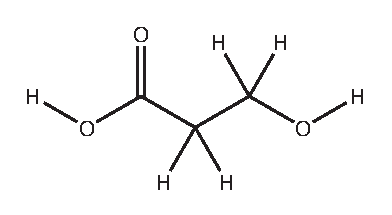
\includegraphics[width=4cm]{figures/propanoic.eps} \end{wrapfigure}
Assuming that the OH group in the carboxylic acid functionalisation will have different forcefield parameters to the primary alcohol at the other end of the molecule, here we must describe the first and second neighbours of the oxygen atoms to differentiate them. \\

To begin, we can describe the carbon atoms as either two or three different types -- either methylene/carboxylic acid, or carboxylic acid/adjacent to a carboxylic acid/adjacent to alcohol. For both, we only need describe the first neighbours of the atoms. For the first:

\begin{verbatim}
    3	C(H2)	C	"nbonds=4,-H,-H,-C"			# Methylene Carbon
    4	C_cbx	C	"nbonds=3,-O(bond=double),-O,-C"	# Carboxylic Acid C
\end{verbatim}

Note the ordering of the oxygen connections for the carboxylic acid carbon, where the most qualified carbon is listed first. This is to stop the doubly-bound oxygen being used to match \qte{--O}, subsequently preventing a successful match. \\

Where all three carbons need to be identified separately, we may write:

\begin{verbatim}
    5	C(OH)	C	"nbonds=4,-H,-H,-C,-O"			# CH2 adjacent to OH
    6	C(COOH)	C	"nbonds=4,-H,-H,-C,-C"			# CH2 adjacent to COOH
    7	C_cbx	C	"nbonds=3,-O(bond=double),-O,-C"	# Carboxylic Acid C
\end{verbatim}

Let us now assume that the hydrogens within the alcohol and carboxylic acid groups must also be seen as different types. In this case, the second neighbours of the atoms must be considered:

\begin{verbatim}
    8	HO	H	"-O(-C(-H,-H))"				# Alcoholic H
    9	H_cbx	H	"-O(-C(-O(bond=double)))"		# Carboxylic acid H
\end{verbatim}

The assignment is thus based entirely on the nature of the carbon atom to which the OH group is bound since this is the next available source of connectivity information. The determination of the three different oxygen atoms is similar:

\begin{verbatim}
    10	OH	O	"-H,-C(-H,-H)"				# Alcoholic O
    11	O_cbx	O	"-C(-O(-H))"				# Carboxylic acid =O
    12	OH_cbx	O	"-H,-C(-O(bond=double))"		# Carboxylic acid O(H)
\end{verbatim}

Of course, we could just have specified \dqte{nbonds=1} for the doubly-bound oxygen of the carboxylic acid group, but that wouldn't be very instructive, would it? 


\subsection{Example 3 -- $N$,$N$,2,5-tetramethylpyridin-4-amine}
\index{typing examples}

\begin{wrapfigure}[]{l}[0em]{3.1cm} 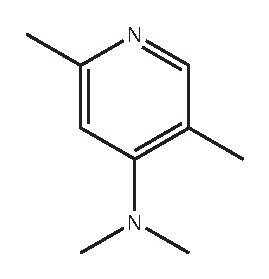
\includegraphics[width=3cm]{figures/aromatic.eps} \end{wrapfigure}
Ah, now here we have a proper problem! An asymmetric substituted pyridine. Lets assume that we need to distinguish between every non-hydrogen atom  -- we'll skip describing the hydrogen atoms for now, but note that this is most easily achieved by specifying directly the atomtype that the H is bound to (see later on). Let's start with the pyridine nitrogen. We basically need to say that its in a 6-membered aromatic ring:

\begin{verbatim}
    13	N_py	N	"ring(size=6,aromatic)"			# Pyridine N
\end{verbatim}


\section{Command Reference}
\label{sec:typingcommands}
\index{typing commands}

All type descriptions in files should be enclosed in double-quotes to prevent delimited parsing of the string. Commands may be separated by spaces or commas, and are case-sensitive. Type descriptions may not span more than one line.

'-' (bound to)
Specifies a connection to another element, but not the exact type of the connection itself (i.e. the bond type, which may be specified with the \qte{bond} keyword in brackets after the element specifier). Immediately following the \qte{--} should be either an element symbol, a type id, or a type name (the last two must be preceeded by a \qte{\$} symbol in order to distinguish them from being plain element symbols). Lists of the elements/type ids/type names may be given in square brackets, separated by commas or spaces, allowing multiple possibilities for matching the connection.

Examples:



bond, sp2, sp3, sp, unbound, geometry, ring (size)


XXX Repetition of descriptions - water example above. The dollar sign.

XXX Type scoring

XXX Art of type writing

XXX Order of atom descriptions


